\documentclass[main]{subfiles}

\begin{document}
    \Date{01.10.19}

    \begin{Task}
      \[F: U \subset \R^2 \ra \R^3,\q C^1 \text{ регулярная}\]
      \begin{figure}[H]
          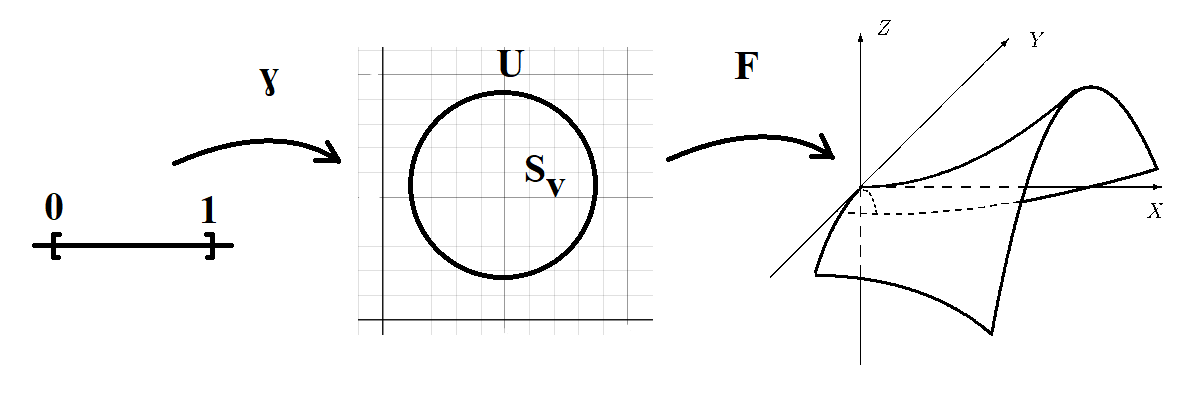
\includegraphics[scale=0.4]{pics/4_1.png}
          \centering
      \end{figure}
      Найти длину $\w{\gamma} = F \circ \gamma$ через $\gamma$ и $\RNumb{1}(F)$
    \end{Task}

    \begin{Sol}
      \[l(F \circ \gamma) := \int_0^1 |F \circ \gamma(t)'| dt\]
      \[\frac{d(F \circ \gamma(t))}{dt} = \ub{\text{вектор}}{\frac{\d F}{\d x}} \ob{\text{скаляр}}{\dot{\gamma_1}(t)}+\frac{\d F}{\d y} \dot{\gamma}_2(t)=\]
      \[=<\frac{\d F}{\d x}\dot{\gamma_1}(t)+\frac{\d F}{\d y} \dot{\gamma}_2(t),\ \frac{\d F}{\d x}\dot{\gamma_1}(t)+\frac{\d F}{\d y} \dot{\gamma}_2(t)>=\]
      \[=<\frac{\d F}{\d x}, \frac{\d F}{\d x}> \dot{\gamma_1^2}(t) + 2<\frac{\d F}{\d x}, \frac{\d F}{\d y}> \dot{\gamma_1}(t)\dot{\gamma_2}(t) + <\frac{\d F}{\d y}, \frac{\d F}{\d y}> \dot{\gamma_2^2}(t)=\]
      \[= (\dot{\gamma_1}, \dot{\gamma_2}) \RNumb{1}(F) \begin{pmatrix}
        \dot{\gamma_1}\\ \dot{\gamma_2}
      \end{pmatrix}\]
      \[\Ra l(F \circ \gamma) = \int_0^1 \sqrt{(\dot{\gamma_1}, \dot{\gamma_2}) \RNumb{1}(F) \begin{pmatrix}
        \dot{\gamma_1}\\ \dot{\gamma_2}
      \end{pmatrix}} dt\]
    \end{Sol}

    \newpage
    \Date{01.10.2019}
    \subsection{Вторая фундаментальная форма}

    \begin{Definition}
      \[F: \us{x,y}{U} \subset \R^2 \ra \R^3 \qq C^2 \text{ регулярная}\]
      \[\abs{\frac{\d F}{\d x} \times \frac{\d F}{\d y}} \neq 0\]
      \[n:=\dfrac{\dfrac{\d F}{\d x} \times \dfrac{\d F}{\d y}}{\abs{\dfrac{\d F}{\d x} \times \dfrac{\d F}{\d y}}} \text{ - перп. обоим и по модулю 1}\]
      \[L=<\frac{\d^2 F}{\d x^2},\ n>,\q
      M=<\frac{\d^2 F}{\d x \d y},\ n>,\q
      N=<\frac{\d^2 F}{\d y^2},\ n>\]
      \[\RNumb{2}(F) = \begin{pmatrix}
        L & M\\
        M & N
      \end{pmatrix}\]
    \end{Definition}

    \begin{Remark}
      \[\RNumb{2}(F) \text{ говорит, какая ПВП лучше всего приближает в данной точке}\]
    \end{Remark}

    \begin{task}
      Пусть есть сфера радиуса r:
      \[\begin{cases}
        x = x_0 + R \cdot \sin \theta\cdot \cos \phi,\\
        y = y_0 + R \cdot \sin \theta\cdot \sin \phi,\\
        z = z_0 + R \cdot \cos \theta,\\
      \end{cases}\]
      где $\theta \in [-\dfrac{\pi}{2},\ \dfrac{\pi}{2}]$ и $\phi \in [0,\ 2\pi)$\\
      Найти $\RNumb{2}(F)$, $\RNumb{1}(F)$ и $\dfrac{\det(\RNumb{2})}{\det(\RNumb{1})}$
    \end{task}

    \begin{sol}
      Посчитаем $\RNumb{1}(F)$:
      \[\frac{\d F}{\d \theta} = (-r \sin\theta \cos\varphi,\ -r \sin\theta \sin\varphi,\ r \cos\theta)\]
      \[\frac{\d F}{\d \varphi} = (-r \cos\theta \sin\varphi,\ r \cos\theta \cos\varphi,\ 0)\]
      \[<\frac{\d F}{\d \theta}, \frac{\d F}{\d \theta}> = r^2,\q
      <\frac{\d F}{\d \theta}, \frac{\d F}{\d \varphi}> = 0\]
      \[<\frac{\d F}{\d \varphi}, \frac{\d F}{\d \theta}> = 0,\q
      <\frac{\d F}{\d \varphi}, \frac{\d F}{\d \varphi}> = r^2 \cos^2 \theta\]
      \[\Ra \RNumb{1}(F) =
      \begin{pmatrix}
        r^2 & 0\\
        0 & r^2 \cos^2 \theta
      \end{pmatrix}\]
      Посчитаем $\RNumb{2}(F)$:
      \[\frac{\d^2 F}{\d \theta^2} = (-r \cos \varphi \cos\theta,\ -r \cos\theta \sin\varphi,\ -r \sin\theta)\]
      \[\frac{\d^2 F}{\d \theta \d\varphi} = (r \sin \theta \sin\varphi,\ -r \sin\theta \cos\varphi,\ 0)\]
      \[\frac{\d^2 F}{\d \varphi^2} = (-r \cos \theta \cos\varphi,\ -r \cos\theta \sin\varphi,\ 0)\]
    \end{sol}

    \begin{reminder}
      В правом ортонормированном базисе:\\
      Если два вектора $\vec{a}$ и $\vec{b}$ представлены координатами
      \[\vec{a} = (a_x,\ a_y,\ a_z),\q \vec{b} = (b_x,\ b_y,\ b_z),\]
      то их векторное произведение имеет координаты
      \[\vec{a} \times \vec{b} = (a_y b_z - a_z b_y,\ a_z b_x - a_x b_z,\ a_x b_y - a_y b_x)\]
      Для запоминания этой формулы удобно использовать мнемонический определитель:
      \[\vec{a} \times \vec{b} =
      \begin{vmatrix}
        \mathbf i & \mathbf j & \mathbf k \\
        a_x & a_y & a_z \\
        b_x & b_y & b_z
      \end{vmatrix},\]
      где $\mathbf i = (1, 0, 0)$, $\mathbf j = (0, 1, 0)$, $\mathbf k = (0, 0, 1)$
    \end{reminder}

    \begin{sol}[продолжение]
      \[\frac{\d F}{\d \theta} \times \frac{\d F}{\d \varphi} =
      (
        -r^2 \cos^2 \theta \cos\varphi,\
        -r^2 \cos^2 \theta \sin\varphi,\
        -r^2 \sin\theta \cos\theta
      )\]
      \[\abs{ \frac{\d F}{\d \theta} \times \frac{\d F}{\d \varphi} } = \r^2 \cos\theta\]

      \[n =
      \dfrac{
        \dfrac{\d F}{\d \theta} \times \dfrac{\d F}{\d \varphi}
      }{
        \abs{\dfrac{\d F}{\d \theta} \times \dfrac{\d F}{\d \varphi}}
      } = (
        - \cos\theta \cos\varphi,\
        -\cos\theta \sin\varphi,\
        -\sin\theta
      )\]
      \[L = <\frac{\d^2 F}{\d \theta^2},\ \ol{n}> = r\]
      \[M = <\frac{\d^2 F}{\d \theta \d \varphi},\ \ol{n}> = 0\]
      \[N = <\frac{\d^2 F}{\d \varphi^2},\ \ol{n}> = r \cos^2 \theta\]
      \[\Ra \RNumb{2}(F) =
      \begin{pmatrix}
        r & 0\\
        0 & r \cos^2 \theta
      \end{pmatrix}\]
      \[K = \frac{\det \RNumb{2}(F)}{\det \RNumb{1}(F)} = \frac{1}{r^2} \text{ - кривизна Гаусса}\]
    \end{sol}

    \begin{task}
      Пусть $\gamma: t \ra (t - \th(t),\ 0,\ \dfrac{1}{\ch(t)}),\q t>0$
      \begin{enumerate}
        \item Найти S поверхности, полученной вращением $\gamma$ вокруг $OZ$
        \item Найти $\RNumb{2}(F)$, $\RNumb{1}(F)$ и $K=\dfrac{\det(\RNumb{2})}{\det(\RNumb{1})}$
      \end{enumerate}
    \end{task}

    \begin{sol}
      Была задача $ (r(t),\ 0,\ z(t)) \Ra (r(t) \cos \varphi,\ r(t)\sin \varphi,\ z(t)),\ \varphi \in [0,\ 2\pi]$\\
      \[\Ra \Br{
        \Br{t - \th(t)}\cos \varphi,\
        \Br{t - \th(t)}\sin \varphi,\
        \dfrac{1}{\ch(t)}},\
      \varphi \in [0,\ 2\pi]\]
      \[\frac{\d F}{\d t} = \Br{
        \Br{1 - \frac{1}{\ch^2(t)}}\cos \varphi,\
        \Br{1 - \frac{1}{\ch^2(t)}}\sin \varphi,\
        \frac{\sh(t)}{\ch^2(t)}
      }\]
      \[\Ra \frac{\d F}{\d t} = \Br{
        \th^2 (t)\cos \varphi,\
        \th^2 (t)\sin \varphi,\
        \frac{\sh(t)}{\ch^2(t)}
      }\]
      \[\frac{\d F}{\d \varphi} = \Br{
        -(t-\th(t))\sin \varphi,\
        (t-\th(t))\cos \varphi,\
        0
      }\]
      \[<\frac{\d F}{\d t}, \frac{\d F}{\d t}> = \th^4 (t)+\frac{\sh^2 (t)}{\ch^4 (t)} = \th^4 \Br{1+\dfrac{1}{\sh^2}} =\th^2 (t),\q
      <\frac{\d F}{\d t}, \frac{\d F}{\d \varphi}> = 0\]
      \[<\frac{\d F}{\d \varphi}, \frac{\d F}{\d t}> = 0,\q
      <\frac{\d F}{\d \varphi}, \frac{\d F}{\d \varphi}> = (t-\th(t))^2 \]
      \[\Ra \RNumb{1}(F) =
      \begin{pmatrix}
        {}\th^2 (t) & 0\\
        0 & (t-\th(t))^2
      \end{pmatrix}\]

      \begin{multline*}
        $$A(S) = \iint \sqrt{\det \RNumb{1}(F)} dt d\varphi =
        \iint \sqrt{(t-\th(t))^2 \th^2 (t)} dt d\varphi =\\
        =\iint \abs{(t-\th(t)) \th (t)} dt d\varphi = \iint (t-\th(t)) \th (t) dt d\varphi$$
      \end{multline*}

      Интеграл не берётся :)

      %\begin{multline*}
      %  $$\dfrac{\d F}{\d t} \times \dfrac{\d F}{\d \varphi} = \\
      %    \Bigg(
      %      \Br{\th^2 (t)\sin \varphi} \Br{0} -
      %        \Br{\frac{\sh(t)}{\ch^2(t)}} \Br{(t-\th(t))\cos \varphi},\ \\
      %      \Br{\frac{\sh(t)}{\ch^2(t)}} \Br{(\th(t)-t)\sin \varphi} -
      %        \Br{\th^2 (t)\cos \varphi} \Br{0},\ \\
      %      \Br{\th^2 (t)\cos \varphi} \Br{(t-\th(t))\cos \varphi}
      %        - \Br{\th^2 (t)\sin \varphi} \Br{(\th(t)-t)\sin \varphi}
      %    \Bigg) =
      %  $$
      %\end{multline*}
      %\begin{multline*}
      %  $$
      %    =\Bigg(
      %      -\Br{\dfrac{\sh(t)}{\ch^2(t)}} (t-\th(t))\cos \varphi,\ \\
      %      \Br{\frac{\sh(t)}{\ch^2(t)}} (\th(t)-t)\sin \varphi,\
      %      (t-\th(t))\th^2 (t)
      %    \Bigg) =
      %  $$
      %\end{multline*}
      %\[\abs{\dfrac{\d F}{\d t} \times \dfrac{\d F}{\d \varphi}} =
      %\sqrt{
      %  \Br{\dfrac{\sh(t)}{\ch^2(t)}} \Br{(t-\th(t))}^2 +
      %  \Br{(t-\th(t))\th^2 (t)}^2
      %}=\]
      %\[=\abs{t-\th(t)} \th^2 (t) \sqrt{\dfrac{1}{\sh^2(t)} + 1} = \abs{(t-\th(t))\th (t)} \th^2 (t) = \th^3 (t) (t-\th(t))\]
      %\[n =
      %\dfrac{
      %  \dfrac{\d F}{\d \theta} \times \dfrac{\d F}{\d \varphi}
      %}{
      %  \abs{\dfrac{\d F}{\d \theta} \times \dfrac{\d F}{\d \varphi}}
      %} = \Br{
      %  -\Br{\dfrac{1}{\ch(t)}} \dfrac{1}{\th^2 (t)} \cos \varphi,\
      %  -\Br{\frac{1}{\ch(t)}} \dfrac{1}{\th^2 (t)} \sin \varphi,\
      %  \dfrac{1}{\th (t)}
      %}
      %\]
      %\[\frac{\d F}{\d t} = \Br{
      %  \th^2 (t)\cos \varphi,\
      %  \th^2 (t)\sin \varphi,\
      %  \frac{\sh(t)}{\ch^2(t)}
      %}\]
      %\[\Ra \frac{\d^2 F}{\d t^2} = \Br{
      %  2 \dfrac{1}{\ch^2 (t)} \th (t) \cos \varphi,\
      %  2 \dfrac{1}{\ch^2 (t)} \th (t) \sin \varphi,\
      %  \dfrac{ch^3 (t) - 2 \sh^2 (t) \ch (t)}{\ch^4 (t)}
      %}\]
      %\[\Ra L = <\frac{\d^2 F}{\d t^2},\ \ol{n}> = ?\]
      %\[\Ra \frac{\d^2 F}{\d t \d \varphi} = \Br{
      %  ?,\
      %  ?,\
      %  ?
      %}\]
      %\[\Ra M = <\frac{\d^2 F}{\d t \d \varphi},\ \ol{n}> = ?\]
      %\[\frac{\d F}{\d \varphi} = \Br{
      %  -(t-\th(t))\sin \varphi,\
      %  (t-\th(t))\cos \varphi,\
      %  0
      %}\]
      %\[\Ra \frac{\d^2 F}{\d \varphi^2} = \Br{
      %  ?,\
      %  ?,\
      %  ?
      %}\]
      %\[\Ra N = <\frac{\d^2 F}{\d \varphi^2},\ \ol{n}> = ?\]
      %\[\Ra \RNumb{2}(F) =
      %\begin{pmatrix}
      %  ? & ?\\
      %  ? & ?
      %\end{pmatrix}\]
      %\[K = \frac{\det \RNumb{2}(F)}{\det \RNumb{1}(F)} = ? \text{ - кривизна Гаусса}\]
    \end{sol}
\end{document}
